\documentclass[12pt, letterpaper]{article}
\usepackage{bbold}
\usepackage{indentfirst}
\usepackage{amsmath, amssymb}
\usepackage[T1]{fontenc}
\usepackage[utf8]{inputenc}
\usepackage{physics}
\usepackage{tensor}
\usepackage{braket}
\usepackage{graphics}
\usepackage{grffile}
\usepackage[export]{adjustbox}
\usepackage{svg}
\usepackage{caption}
\usepackage{subcaption}
\usepackage{authblk} 
\usepackage{blindtext}
\usepackage{setspace}
\usepackage{xcolor}
\usepackage{tcolorbox}
\usepackage{listings}
\usepackage[framemethod=TikZ]{mdframed}
\mdfdefinestyle{MyFrame}{%
    linecolor=black,
    outerlinewidth=2pt,
    roundcorner=20pt,
    innertopmargin=\baselineskip,
    innerbottommargin=\baselineskip,
    innerrightmargin=20pt,
    innerleftmargin=20pt,
    backgroundcolor=gray!50!white}
\title{}

\begin{document}
    \section*{Report On Using MCMC Method To Find Hamiltonian And Thermalizaion of Berry-Keating And Damped Harmonic Oscillator}
    \subsection*{Preliminaries}
        Hamiltonian of Berry-Keating  
        \begin{equation}
            H = \frac{1}{2}(xp + px)
        \end{equation}
        \\
        
    

        We're using MCMC method to evaluate Hamiltonian and Thermalization of Berry-Keating. 
    
    \subsection*{Methodology}
        Markov Chain Monte Carlo (MCMC) is a random sampling method to visit x with a probability proportional to some given
        distribution say, $\pi (x)$. To use MCMC in simulation we first simplify the Hamiltonian Monte Carlo code in a block
        manner. Then we calculate and plot $<H>$ graphs of Berry-Keating Hamiltonian. 
        But first simplify code using header files. Those codes are giiven below
        \begin{mdframed}[style=MyFrame]
            \subsection*{matrix.h}
            \begin{verbatim}
#ifndef MATRIX
#define MATRIX
#include<complex>
using namespace std;
const int n=10;
/* 
    Declaring a function for easily calling a matrix, it 2nd, 
    3rd, 4th order terms, and their traces.
*/
double matrix(complex<double> A[n][n], complex<double> 
(&A2)[n][n], complex<double> (&A3)[n][n], complex<double> 
(&A4)[n][n], double& s, double& s2, double& s3, double& s4)
{
    s=0, s2=0, s3=0, s4=0;

    // 2nd Order matrix
    for(int i=0; i<n; i+=1)
    {
        for(int j=0; j<n; j+=1)
        {
            for(int k=0; k<n; k+=1)
            {
                A2[i][j] += A[i][k]*A[k][j];
            }
        }
    }

    //  3rd order matrix
    for(int i=0; i<n; i+=1)
    {
        for(int j=0; j<n; j+=1)
        {
            for(int k=0; k<n; k+=1)
            {
                A3[i][j] += A2[i][k]*A[k][j];
            }
        }
    }
    
    // 4th order matrix
    for(int i=0; i<n; i+=1)
    {
        for(int j=0; j<n; j+=1)
        {
            for(int k=0; k<n; k+=1)
            {
                A4[i][j] += A3[i][k]*A[k][j];
            }
        }
    }

    //  Trace of A
    for(int i=0; i<n; i+=1)
    {
        s += A[i][i].real();
    }

    // Trace of A^2
    for(int i=0; i<n; i+=1)
    {
        s2 += A2[i][i].real();
    }
    
    //  Trace of A^3
    for(int i=0; i<n; i+=1)
    {
        s3 += A3[i][i].real();
    }
    
    //  Trace of A^4
    for(int i=0; i<n; i+=1)
    {
        s4 += A4[i][i].real();
    }
    
    return 0;
}

#endif
            \end{verbatim}        
        \end{mdframed}

        \begin{mdframed}[style=MyFrame]
        \subsection*{box.h}
        \begin{verbatim}
            #ifndef BOX
            #define BOX

            #include<cstdlib>
            #include<cmath>
            
            double Box(double& x, double& y)
            {
                double p,q;

                p = (double)rand()/(double)RAND_MAX;
                q = (double)rand()/(double)RAND_MAX;

                x = sqrt(-2*log(p))*sin(2*M_PI*q);
                y = sqrt(-2*log(p))*cos(2*M_PI*q);

                return 0;
            }

            #endif.
        \end{verbatim}        
    \end{mdframed}

    \begin{mdframed}[style=MyFrame]
        \subsection*{hamiltonian.h}
        \begin{verbatim}
        
#ifndef HAM
#define HAM

/* 
    Calculating Hamiltonian of Berry-Keating H = 
    (1/2)(xp+px)
*/
double hamiltonian(complex<double> A[n][n], 
complex<double> B[n][n])
{
    complex <double> H[n][n] = {0}, N1[n][n] = {0}, 
    N2[n][n] = {0};
    double sum=0;

    for(int i=0; i<n; i+=1)
    {
        for(int j=0; j<n; j+=1)
        {
            for(int k=0; k<n; k+=1)
            {
                N1[i][j] += A[i][k]*B[k][j];
            }
        }
    }

    for(int i=0; i<n; i+=1)
    {
        for(int j=0; j<n; j+=1)
        {
            for(int k=0; k<n; k+=1)
            {
                N2[i][j] += B[i][k]*A[k][j];
            }
        }
    }

    for(int i=0; i<n; i+=1)
    {
        for(int j=0; j<n; j+=1)
        {
            H[i][j] = N1[i][j] + N2[i][j];
        }
    }

    for(int i=0; i<n; i+=1)
    {
        sum += H[i][i].real();
    }

    return 0.5*sum;
}

#endif

        \end{verbatim}        
    \end{mdframed}

    \begin{mdframed}[style=MyFrame]
        \subsection*{force.h}
        \begin{verbatim}
            #ifndef FORCE
#define FORCE

#include<matrix.h>


/* 
    Calculating force (dH/d phi = dS/d phi) term = p
*/
double force(complex<double> A[n][n], 
complex<double> (&dh)[n][n])
{
    // calculating force matrix
    for(int i=0; i<n; i+=1)
    {
        for(int j=0; j<n; j+=1)
        {
            dh[i][j] = (A[i][j]); 
        }
    }

    return 0;
}

#endif
        \end{verbatim}        
    \end{mdframed}

    \begin{mdframed}[style=MyFrame]
        \subsection*{molecular.h}
        \begin{verbatim}
#ifndef MOL
#define MOL

#include<box.h>
#include<force.h>
#include<hamiltonian.h>
/*
    Molecular dynamics part
*/
double molecular(complex<double> (&phi)[n][n], 
complex<double> (&P)[n][n], double& hi, double& hf)
{
    double p, q, r1, r2,nt=10; 

    complex<double>  dt=0.01, dh[n][n] = {0};

    for(int i=0; i<n; i+=1)
    {
        for(int j=0; j<n; j+=1)
        {   
            Box(p,q);
            P[i][j] = complex(p/sqrt(2),q/sqrt(2));
        }
    }

    // Initial hamiltonian of molecular dynamics
    hi = hamiltonian(phi,P);


    //leap frog method 
    // xi(dt/2) = xi(0) + pi(0)dt/2;
    for(int i=0; i<n; i+=1)
    {
        for(int j=0; j<n; j+=1)
        {
            phi[i][j] += 0.5*P[i][j]*dt;
        }
    }

    // for n=1 to nt steps
    //pi(ndt) = pi((n-1)dt) - (ds/dx)((n-1/2)dt)dt
    for(int i=1; i<=nt-1; i+=1)
    {
        //calling force term
        force(P,dh);
        for(int j=0; j<n; j+=1)
        {
            for(int k=0; k<n; k+=1)
            {
                P[j][k] -= dh[j][k]*dt;
                phi[j][k] += P[j][k]*dt;
            }
        }
    }
    
    //calling force term
    //late step of leap frog method
    //pi(nt *dt) = pi((nt-1)dt) -  (ds/dx)((nt-1/2)dt)dt
    //xi(nt* dt) = xi((nt-1)dt) + p(nt *dt) dt/2;
    force(P,dh);
    for(int i=0; i<n; i+=1)
    {
        for(int j=0; j<n; j+=1)
        {
            P[i][j] -= dh[i][j]*dt;
            phi[i][j] += 0.5*P[i][j]*dt;
        }
    }

    //final hamiltonian of molecular dynamics
    hf = hamiltonian(phi,P);

    return 0;
}

#endif
        \end{verbatim}        
    \end{mdframed}

    \begin{mdframed}[style=MyFrame]
        \subsection*{main.cpp}
        \begin{verbatim}
#include<box.h>
#include<force.h>
#include<molecular.h>
#include<matrix.h>
#include<iostream>
#include<cmath>
#include<fstream>
#include<cstdlib>
#include<complex>
#include<ctime>
using namespace std;

double fact(double x)
{
    double s=1;
    for(int i=1; i<=x; i+=1)
    {
        s *= i*(i+1);
    }

    return s;
}

int main()
{
    srand(time(NULL));
    ofstream fout("main.dat");
    ofstream file("part.dat");
    double hi, hf, s=0, s2=0, r, 
    c=0,p,q,C[10000]={},x=0,a=0, D[10000][10]={};
    long double x1=0, x2, y1=0, y2=0;
    const int n=10;
    double t = 198;
    //x=0;
    complex<double> A[n][n] = {0}, 
    A0[n][n] = {0},B[n][n] = {0},B0[n][n] = {0};

        
        //t += 1000;
        //generating random value for x
        for(int i=0; i<n; i+=1)
        {
            for(int j=0; j<n; j+=1)
            {   
                p=(double)rand()/(double)RAND_MAX;
                q=(double)rand()/(double)RAND_MAX;
                A[i][j]=complex(p,q);
            }
        }

        //metropolis test
        for(int i=1; i<10000; i+=1)
        {
            for(int j=0; j<n; j+=1)
            {
                for(int k=0; k<n; k+=1)
                {   
                    //x0=x
                    A0[j][k] = A[j][k];

                }
            }
            
            molecular(A,B,hi,hf);
            r = (double)rand()/(double)RAND_MAX;
            if(exp(hi-hf)>r)
            {
                c+=1;
            }

            else
            {
                for(int j=0; j<n; j+=1)
                {
                    for(int k=0; k<n; k+=1)
                    {
                        A[j][k] = A0[j][k];
                    }
                }
            }

            s = hamiltonian(A,B);
            s2 += hamiltonian(A,B);
            C[i] = s;
            fout << i << "  " << (double)s/(double)i 
            << "  " << (double)s2/(double)(i) << endl;
        }

        //calculating partition function
        y1=0, x1=0;
        for(int i=1; i<10000; i+=1)
        {
            y1 += exp(-C[i]/t);

        }

        // sum of <H>*exp(-\beta H)/Z 
        for(int i=1; i<10000; i+=1)
        {
            x1 += C[i]*exp(-C[i]/t);
            // D[i][l] = x1/y1;

            file << i << "  " << x1/y1 << endl;

        }



    return 0;
}
        \end{verbatim}        
    \end{mdframed}

        \begin{adjustbox}{center,caption={Graph of Expectation value of Berry-Keating},nofloat=figure,label={somelabel}}
            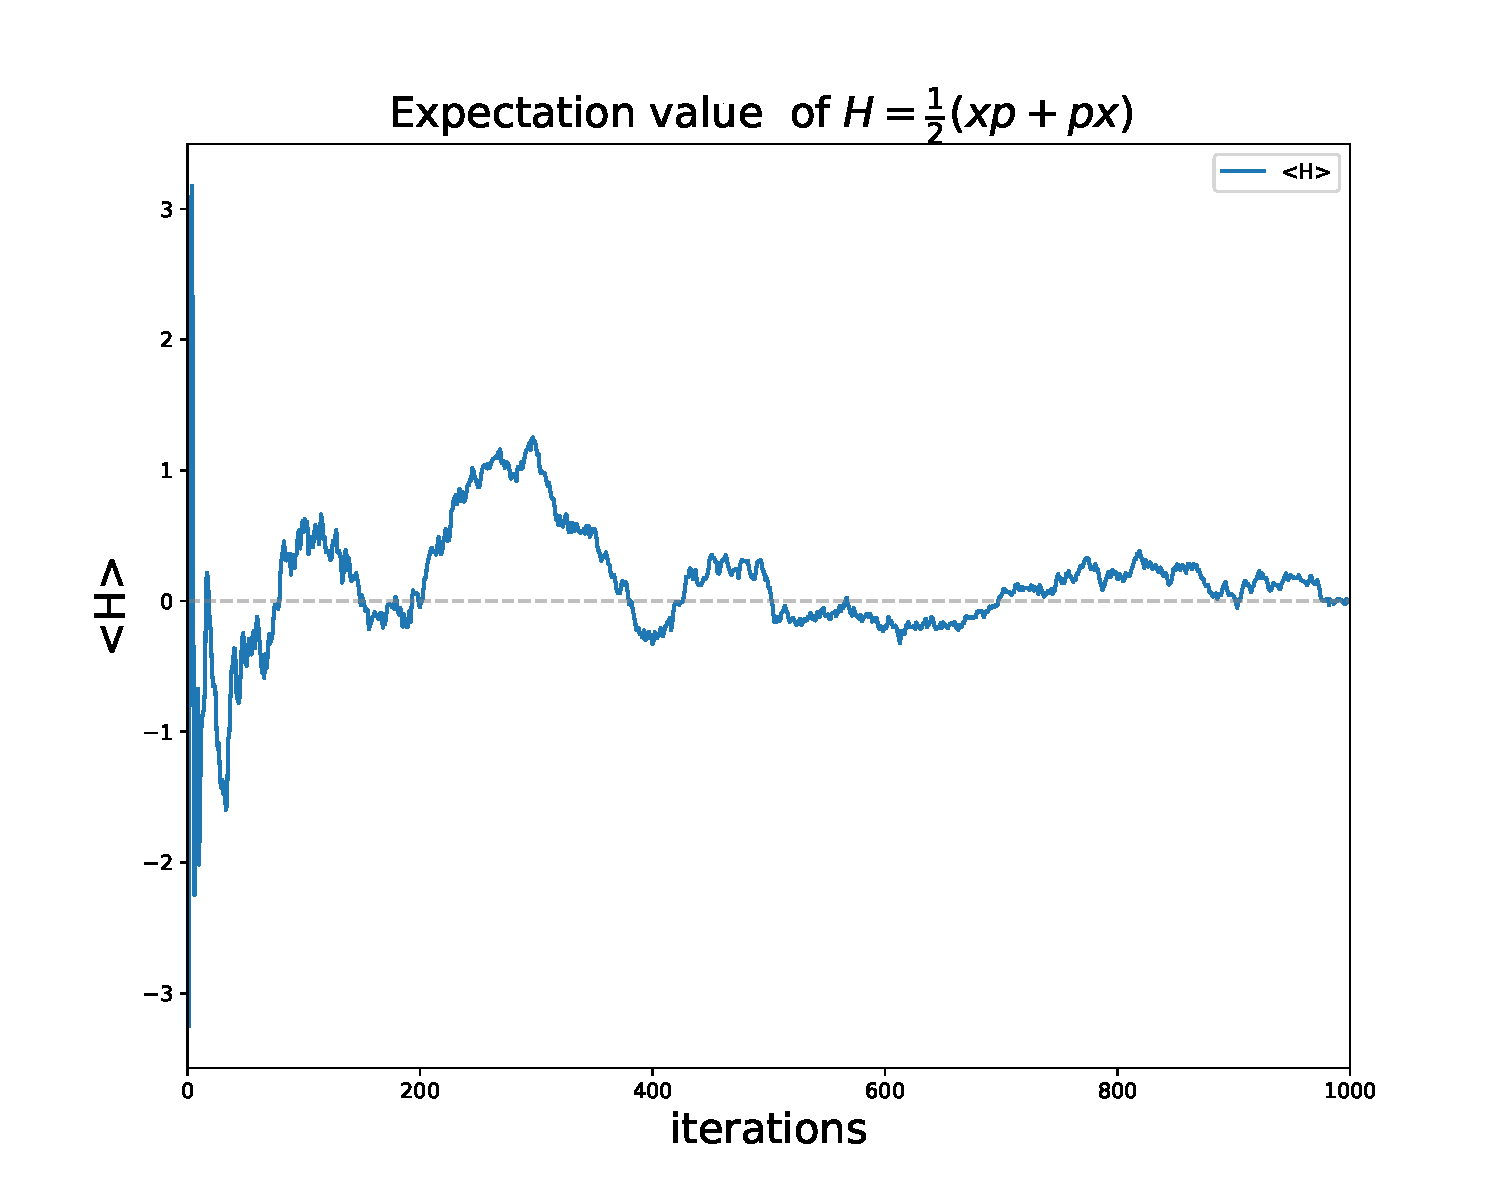
\includegraphics[width=0.8\textwidth]{bk.pdf}
        \end{adjustbox}

        Again evaluating $<H>$ using probability function where

        \begin{equation}
            <H> = Tr (\frac{\hat{H}*exp(-\beta \hat{H})}{Tr (exp(-\beta \hat{H} ))})
        \end{equation}
        \begin{adjustbox}{center,caption={Graph of Expectation value of Berry-Keating},nofloat=figure,label={somelabel}}
            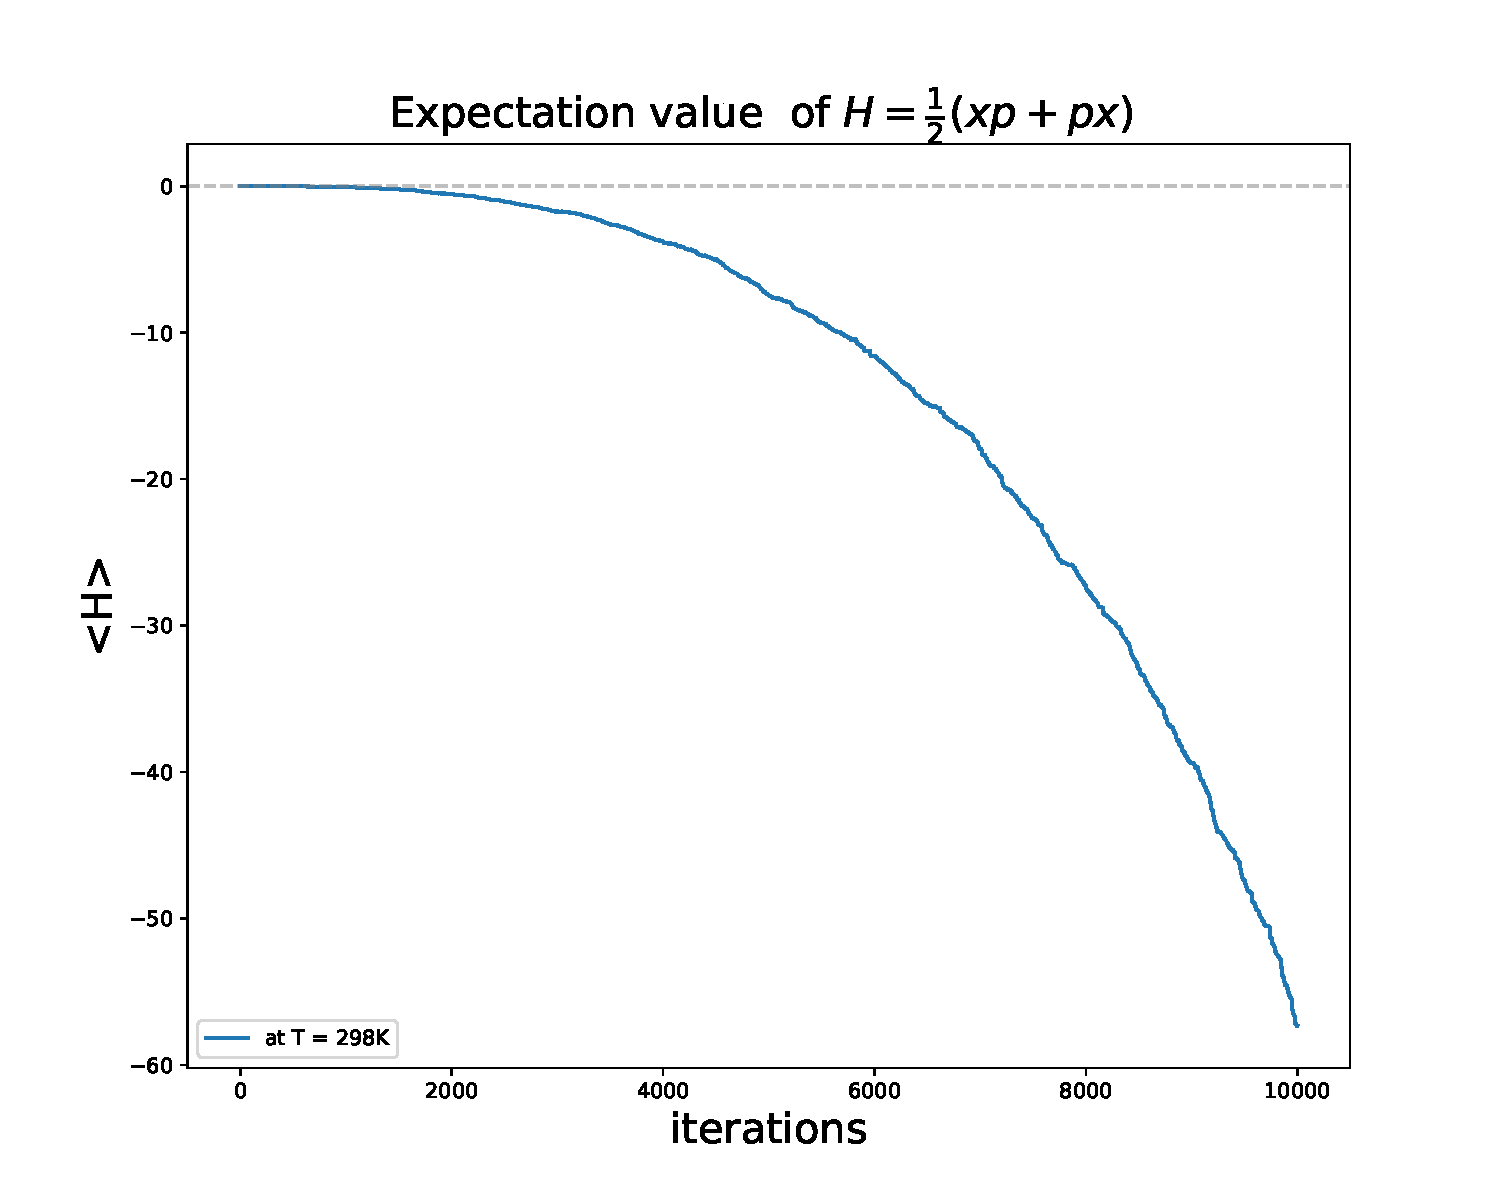
\includegraphics[width=0.8\textwidth]{beta.pdf}
        \end{adjustbox}
\end{document}